\documentclass[border=12pt,tikz]{standalone}
\usepackage{helvet}
\renewcommand{\familydefault}{\sfdefault}
\usepackage{amsmath}
\usepackage{tikz}
\usepackage{tikz-3dplot}
\usetikzlibrary{calc,positioning,shapes.geometric,arrows.meta,decorations.pathreplacing,backgrounds}

% Volume Palette Colors
\definecolor{emeraldpine}{HTML}{1A4D3E}
\definecolor{harvardcrimson}{HTML}{A51C30}
\definecolor{ethdarkblue}{HTML}{1F407A}
\definecolor{ethpetrol}{HTML}{007A87}
\definecolor{ethbronze}{HTML}{B87333}
\definecolor{ink}{HTML}{1A202C}
\definecolor{softink}{HTML}{4A5568}
\definecolor{paleink}{HTML}{CBD5E1}
\definecolor{cardbg}{HTML}{F8FAFC}
\definecolor{shadecolor}{HTML}{F1F5F9}

\begin{document}
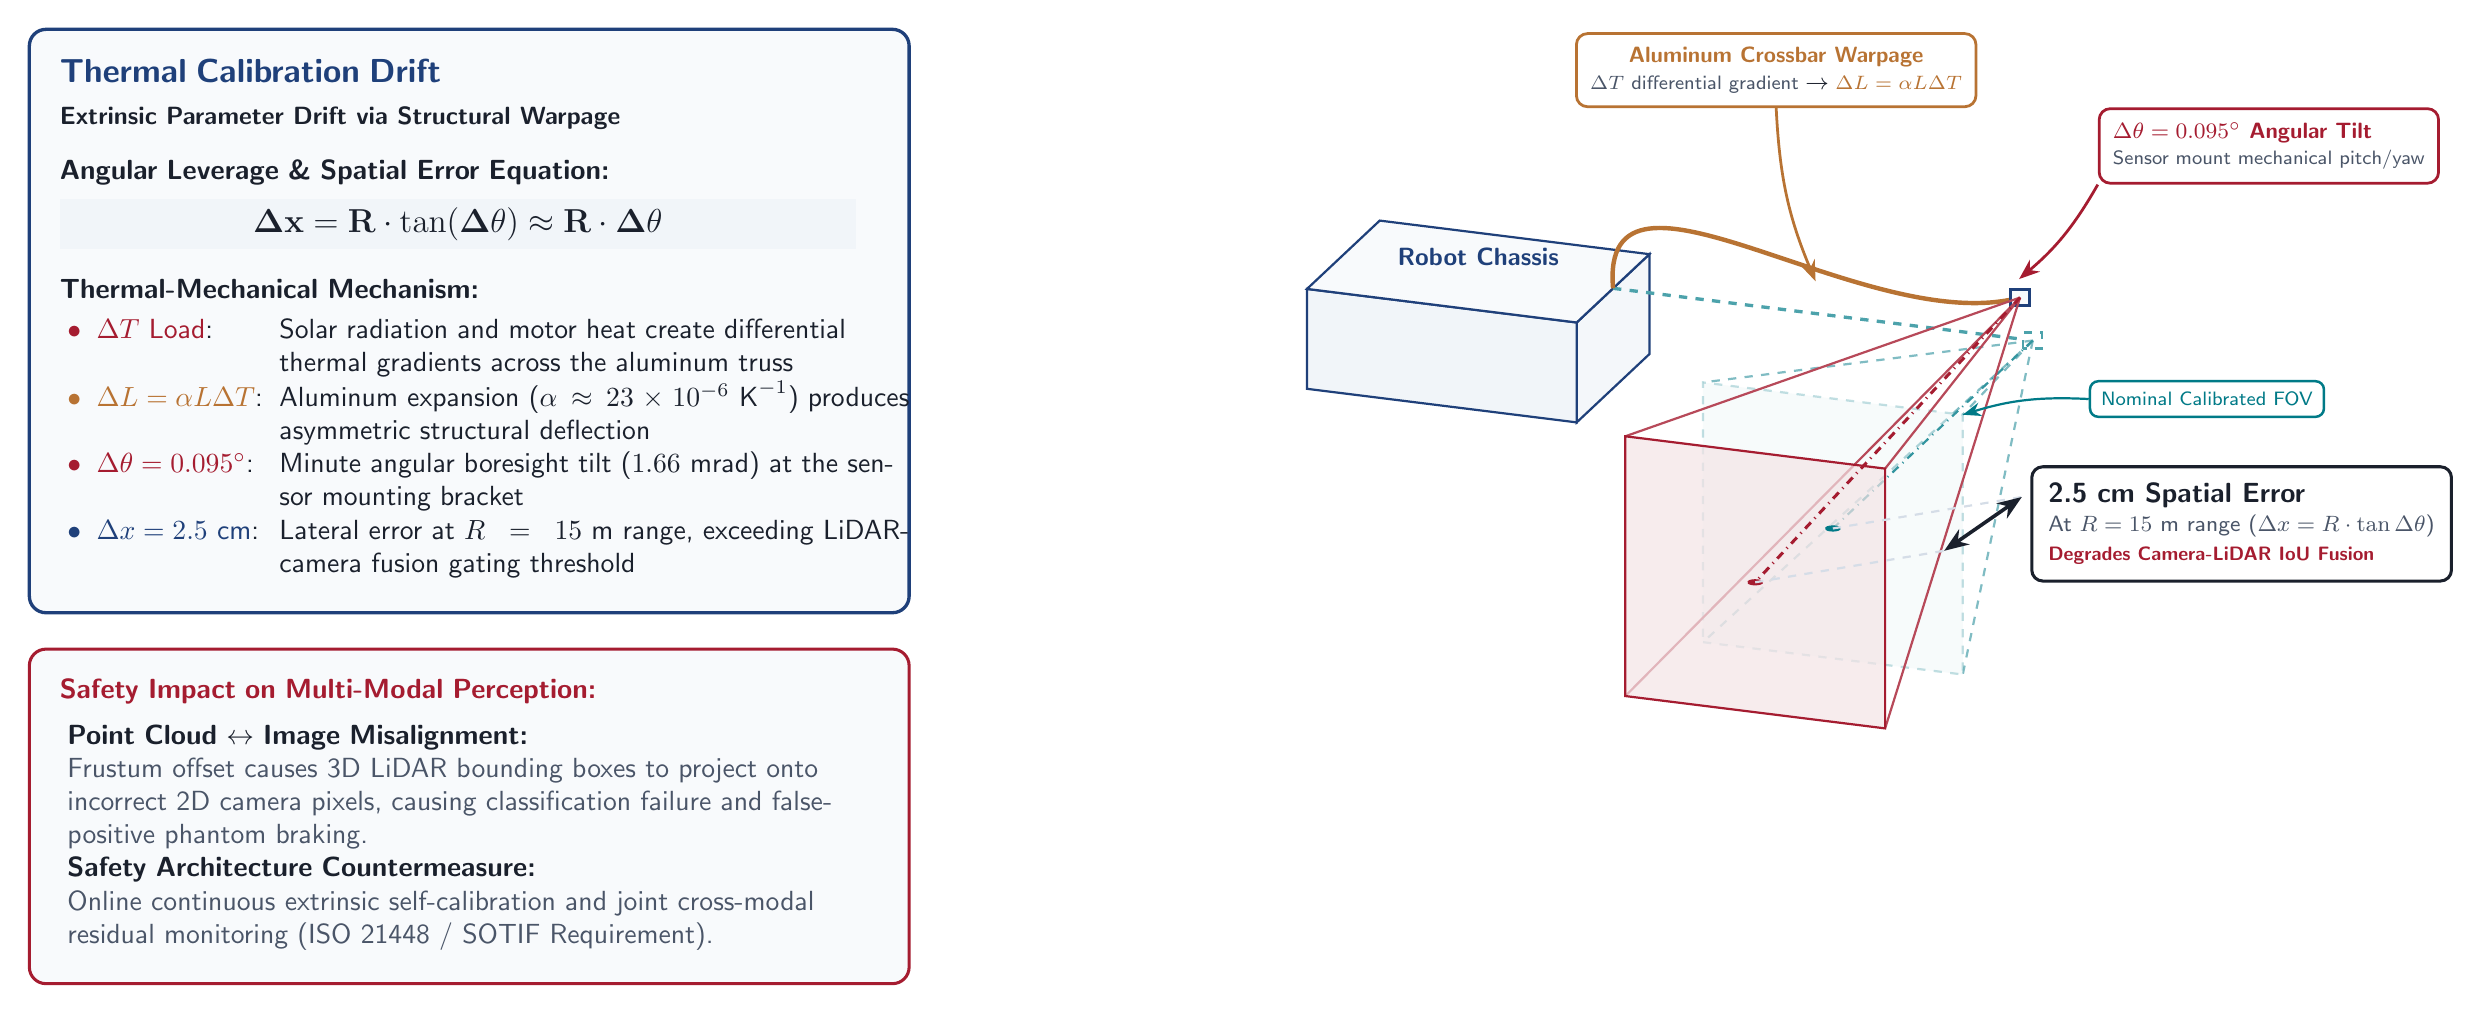
\begin{tikzpicture}[font=\sffamily, >=Stealth]
    
    % ==========================================================
    % LEFT COLUMN: THEORY & SPECIFICATION CARDS (2D canvas)
    % ==========================================================
    \node[anchor=north west, fill=cardbg, draw=ethdarkblue, line width=1.2pt, rounded corners=6pt, inner sep=11pt, text=ink, text width=10.4cm] (theoryCard) at (0, 0) {
        {\large\bfseries\textcolor{ethdarkblue}{Thermal Calibration Drift}}\\[3pt]
        {\small\bfseries Extrinsic Parameter Drift via Structural Warpage}\\[8pt]
        \textbf{Angular Leverage \& Spatial Error Equation:}\\[4pt]
        \colorbox{shadecolor}{\parbox{9.9cm}{\centering\large $\mathbf{\Delta x = R \cdot \tan(\Delta\theta) \approx R \cdot \Delta\theta}$}}\\[10pt]
        {\bfseries Thermal-Mechanical Mechanism:}\\[5pt]
        \begin{tabular}{@{\;}l@{\hspace{6pt}}p{8.0cm}@{}}
        \textcolor{harvardcrimson}{$\bullet$\;\;$\Delta T$ Load}: & Solar radiation and motor heat create differential thermal gradients across the aluminum truss \\
        \textcolor{ethbronze}{$\bullet$\;\;$\Delta L = \alpha L \Delta T$}: & Aluminum expansion ($\alpha \approx 23 \times 10^{-6}\text{ K}^{-1}$) produces asymmetric structural deflection \\
        \textcolor{harvardcrimson}{$\bullet$\;\;$\Delta\theta = 0.095^\circ$}: & Minute angular boresight tilt ($1.66\text{ mrad}$) at the sensor mounting bracket \\
        \textcolor{ethdarkblue}{$\bullet$\;\;$\Delta x = 2.5\text{ cm}$}: & Lateral error at $R = 15\text{ m}$ range, exceeding LiDAR-camera fusion gating threshold
        \end{tabular}
    };

    \node[anchor=north west, fill=cardbg, draw=harvardcrimson, line width=1.1pt, rounded corners=6pt, inner sep=11pt, text=ink, text width=10.4cm, below=12pt of theoryCard] (impactCard) {
        {\bfseries\textcolor{harvardcrimson}{Safety Impact on Multi-Modal Perception:}}\\[5pt]
        \begin{tabular}{@{\;}p{9.9cm}@{}}
        \textbf{Point Cloud $\leftrightarrow$ Image Misalignment:}\newline
        \textcolor{softink}{Frustum offset causes 3D LiDAR bounding boxes to project onto incorrect 2D camera pixels, causing classification failure and false-positive phantom braking.}\\[5pt]
        \textbf{Safety Architecture Countermeasure:}\newline
        \textcolor{softink}{Online continuous extrinsic self-calibration and joint cross-modal residual monitoring (ISO 21448 / SOTIF Requirement).}
        \end{tabular}
    };

    % ==========================================================
    % RIGHT COLUMN: 3D SPATIAL DRIFT VISUALIZATION
    % ==========================================================
    \tdplotsetmaincoords{70}{110}
    \begin{scope}[shift={(19.5, -4.5)}, scale=1.35, tdplot_main_coords]
        
        % Chassis dimensions
        \def\chMinX{-1.0}
        \def\chMaxX{1.0}
        \def\chMinY{-2.2}
        \def\chMaxY{0.5}
        \def\chH{1.0}

        % Chassis Box
        % Rear face
        \draw[thick, fill=shadecolor!80, draw=ethdarkblue] (\chMinX, \chMaxY, 0) -- (\chMaxX, \chMaxY, 0) -- (\chMaxX, \chMaxY, \chH) -- (\chMinX, \chMaxY, \chH) -- cycle;
        % Right face
        \draw[thick, fill=shadecolor, draw=ethdarkblue] (\chMaxX, \chMinY, 0) -- (\chMaxX, \chMaxY, 0) -- (\chMaxX, \chMaxY, \chH) -- (\chMaxX, \chMinY, \chH) -- cycle;
        % Top face
        \draw[thick, fill=cardbg, draw=ethdarkblue] (\chMinX, \chMinY, \chH) -- (\chMaxX, \chMinY, \chH) -- (\chMaxX, \chMaxY, \chH) -- (\chMinX, \chMaxY, \chH) -- cycle;

        % Chassis label on top face
        \node[ethdarkblue, font=\bfseries\small] at (0, -0.85, \chH + 0.15) {Robot Chassis};

        % Crossbar base at top corner
        \coordinate (CBBase) at (0, 0.5, \chH);
        \def\cbL{4.2}
        \coordinate (CBEndOrig) at (0, 0.5+\cbL, \chH);
        \coordinate (CBEndWarp) at (0.35, 0.5+\cbL, \chH + 0.55);

        % Original straight crossbar
        \draw[very thick, ethpetrol!70, dashed] (CBBase) -- (CBEndOrig);

        % Thermally warped crossbar
        \draw[ultra thick, ethbronze] (CBBase) to[out=95, in=195] (CBEndWarp);

        % Sensor bracket & housings
        % Nominal sensor (dashed)
        \draw[thick, ethpetrol!70, dashed, fill=white] ($(CBEndOrig)+(-0.15,-0.15,-0.15)$) rectangle ($(CBEndOrig)+(0.15,0.15,0.15)$);
        % Warped sensor (solid)
        \draw[thick, ethdarkblue, fill=cardbg] ($(CBEndWarp)+(-0.15,-0.15,-0.15)$) rectangle ($(CBEndWarp)+(0.15,0.15,0.15)$);

        % Frustums
        \def\fL{5.5}
        \def\fW{1.3}

        % 1. NOMINAL FRUSTUM (ethpetrol / cyan)
        \coordinate (FO) at (CBEndOrig);
        \coordinate (FE1) at ($(FO) + (\fL, -\fW, -\fW)$);
        \coordinate (FE2) at ($(FO) + (\fL, \fW, -\fW)$);
        \coordinate (FE3) at ($(FO) + (\fL, \fW, \fW)$);
        \coordinate (FE4) at ($(FO) + (\fL, -\fW, \fW)$);
        \coordinate (FC)  at ($(FO) + (\fL, 0, 0)$);

        \draw[thick, ethpetrol!50, dashed] (FO) -- (FE1);
        \draw[thick, ethpetrol!50, dashed] (FO) -- (FE2);
        \draw[thick, ethpetrol!50, dashed] (FO) -- (FE3);
        \draw[thick, ethpetrol!50, dashed] (FO) -- (FE4);
        \draw[thick, ethpetrol!60, dashed, fill=ethpetrol!8, opacity=0.4] (FE1) -- (FE2) -- (FE3) -- (FE4) -- cycle;
        \draw[ethpetrol!80, dash dot, thick] (FO) -- (FC);

        % 2. WARPED / DRIFTED FRUSTUM (harvardcrimson)
        \coordinate (FW) at (CBEndWarp);
        \coordinate (FWC) at ($(FW) + (\fL, -0.65, -1.05)$);
        \coordinate (FWE1) at ($(FWC) + (0, -\fW, -\fW)$); 
        \coordinate (FWE2) at ($(FWC) + (0, \fW, -\fW)$);
        \coordinate (FWE3) at ($(FWC) + (0, \fW, \fW)$);
        \coordinate (FWE4) at ($(FWC) + (0, -\fW, \fW)$);

        \draw[thick, harvardcrimson!80] (FW) -- (FWE1);
        \draw[thick, harvardcrimson!80] (FW) -- (FWE2);
        \draw[thick, harvardcrimson!80] (FW) -- (FWE3);
        \draw[thick, harvardcrimson!80] (FW) -- (FWE4);
        \draw[thick, harvardcrimson, fill=harvardcrimson!12, fill opacity=0.7] (FWE1) -- (FWE2) -- (FWE3) -- (FWE4) -- cycle;
        \draw[harvardcrimson, dash dot, line width=1.1pt] (FW) -- (FWC);

        % Center points markers
        \filldraw[ethpetrol] (FC) circle (0.07);
        \filldraw[harvardcrimson] (FWC) circle (0.07);

        % 3D Targets for 2D callouts
        \coordinate (tgtCrossbar) at (0.2, 0.5+\cbL*0.5, \chH+0.4);
        \coordinate (tgtTilt) at ($(CBEndWarp)+(0.3, 0.1, 0.3)$);
        \coordinate (tgtFC) at (FC);
        \coordinate (tgtFWC) at (FWC);
        \coordinate (tgtFE3) at (FE3);
        \coordinate (tgtFWE3) at (FWE3);
    \end{scope}

    % ==========================================================
    % CALLOUTS & SPATIAL ERROR DIMENSION (2D canvas)
    % ==========================================================
    % Crossbar Callout (top)
    \node[anchor=south, fill=white, draw=ethbronze, line width=1pt, rounded corners=4pt, inner sep=5pt, font=\footnotesize, text=ink, align=center] 
        (calloutBar) at ([shift={(-0.5cm, 2.2cm)}]tgtCrossbar) {
            \textcolor{ethbronze}{\bfseries Aluminum Crossbar Warpage}\\
            \textcolor{softink}{\scriptsize $\Delta T$ differential gradient}\;$\rightarrow$\;\textcolor{ethbronze}{\scriptsize $\Delta L = \alpha L \Delta T$}
        };
    \draw[->, line width=1pt, ethbronze] (calloutBar.south) to[bend right=10] (tgtCrossbar);

    % Angular Tilt Callout
    \node[anchor=south west, fill=white, draw=harvardcrimson, line width=1pt, rounded corners=4pt, inner sep=5pt, font=\footnotesize, text=ink, align=left] 
        (calloutTilt) at ([shift={(1.0cm, 1.2cm)}]tgtTilt) {
            \textcolor{harvardcrimson}{\bfseries $\Delta\theta = 0.095^\circ$ Angular Tilt}\\
            \textcolor{softink}{\scriptsize Sensor mount mechanical pitch/yaw}
        };
    \draw[->, line width=1pt, harvardcrimson] (calloutTilt.south west) to[bend left=10] (tgtTilt);

    % Nominal FOV label
    \node[anchor=west, fill=white, draw=ethpetrol, line width=0.9pt, rounded corners=3pt, inner sep=4pt, font=\scriptsize, text=ethpetrol] 
        (calloutNominal) at ([shift={(1.6cm, 0.2cm)}]tgtFE3) {Nominal Calibrated FOV};
    \draw[->, line width=0.8pt, ethpetrol] (calloutNominal.west) to[bend right=10] (tgtFE3);

    % Dimension extension lines and arrow OUTSIDE the frustum (shifted right by 2.4cm)
    \coordinate (extOrig) at ([shift={(2.4cm, 0.4cm)}]tgtFC);
    \coordinate (extWarp) at ([shift={(2.4cm, 0.4cm)}]tgtFWC);
    \draw[paleink!80, line width=0.8pt, dashed] (tgtFC) -- (extOrig);
    \draw[paleink!80, line width=0.8pt, dashed] (tgtFWC) -- (extWarp);
    \draw[<->, line width=1.3pt, ink] (extOrig) -- (extWarp);

    % Spatial Error at 15m Callout (Placed cleanly next to dimension line)
    \node[anchor=west, fill=white, draw=ink, line width=1.1pt, rounded corners=4pt, inner sep=6pt, font=\footnotesize, text=ink, align=left] 
        (calloutErr) at ([shift={(0.6cm, 0cm)}]$0.5*(extOrig)+0.5*(extWarp)$) {
            \textbf{\normalsize 2.5 cm Spatial Error}\\[1pt]
            \textcolor{softink}{\footnotesize At $R = 15\text{ m}$ range ($\Delta x = R \cdot \tan\Delta\theta$)}\\[1pt]
            \textcolor{harvardcrimson}{\bfseries\scriptsize Degrades Camera-LiDAR IoU Fusion}
        };

\end{tikzpicture}
\end{document}
